The interface subsystems of the RoamBot are responsible for processing user input and translating it into commands for the rover. These subsystems are implemented using C, C++, and Python and operate on the Raspberry Pi 5.

%In this section, the layer is described in terms of the hardware and software design. Specific implementation details, such as hardware components, programming languages, software dependencies, operating systems, etc. should be discussed. Any unnecessary items can be ommitted (for example, a pure software module without any specific hardware should not include a hardware subsection). The organization, titles, and content of the sections below can be modified as necessary for the project.

\subsection{Layer Hardware}
The Raspberry Pi 5 serves as the core interface hardware for the RoamBot, providing robust computational power with its quad-core ARM Cortex-A76 processor and 16GB of LPDDR4x RAM. It efficiently handles real-time pathfinding and decision-making processes. Additionally, its USB 3.0 ports and GPIO pins allow for direct connection to sensors and motor controllers.
%%%%%%%%%%%%%%% DEFINE MORE HARDWARE

\subsection{Layer Operating System}
The operating system used for the interface layer is Ubuntu 24.04, providing a stable environment for development and execution.

\subsection{Layer Software Dependencies}
The interface subsystems rely on the ROS2 framework for robotic control. These libraries are utilized for implementing communication protocols, control algorithms, and user input processing.

\subsubsection{Layer Programming Languages}
This layer is implemented using C, C++, and Python to efficiently process user commands and algorithm decisions and communicate with the motor control system.

\newpage

\subsection{UI Control}
The UI control subsystem serves as the top-level software interface for managing user interactions. It enables switching between direct user control and automated algorithmic control.

\begin{figure}[h!]
	\centering
 	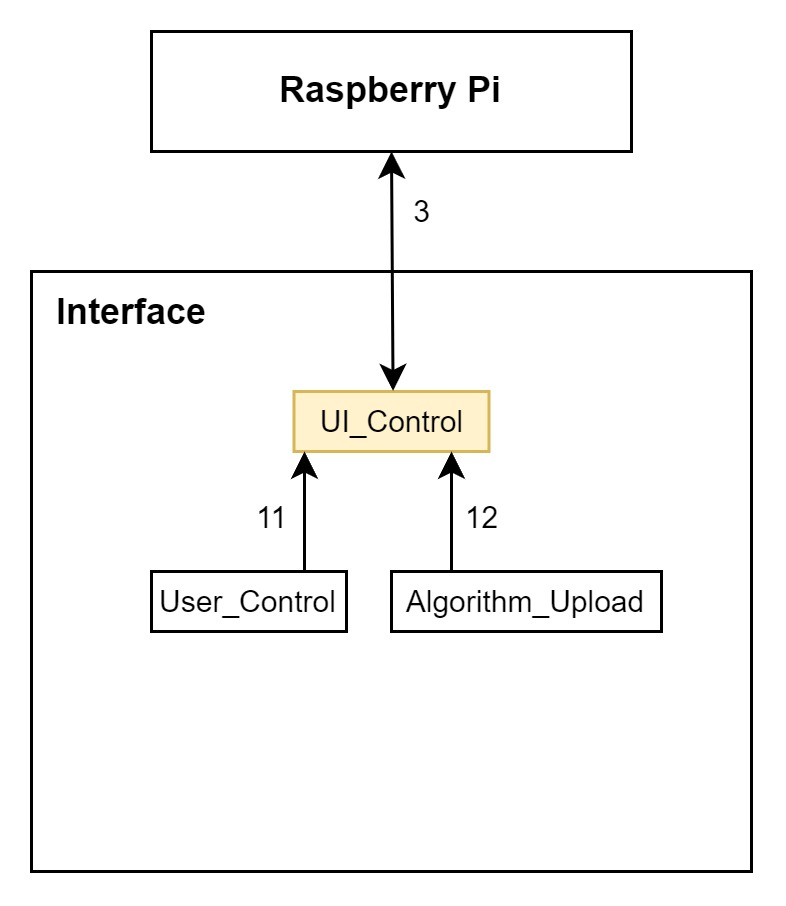
\includegraphics[width=0.60\textwidth]{images/interface/1_ui.jpg}
 \caption{Interface Layer - UI Control Subsystem}
\end{figure}

\subsubsection{Subsystem Data Structures}
The subsystem uses flag-based data structures to manage control mode status, with flags indicating whether the rover is in manual or autonomous mode. These flags are checked in real-time to determine which set of functions or commands should be executed.

\subsubsection{Subsystem Data Processing}
The UI control subsystem processes incoming user commands to switch between manual and automated modes by interpreting the mode. When a switch occurs, the system either routes input to the manual control system, allowing the user to directly guide the rover, or to the autonomous system, where the rover executes pre-programmed algorithms.

\newpage

\subsection{User Control}
The User Control subsystem allows direct manipulation of the RoamBot's movement in real-time. It processes immediate user inputs, and translates the input into motion instructions. This subsystem ensures that users have precise control over speed and direction, allowing manual operation when needed.

\begin{figure}[h!]
	\centering
 	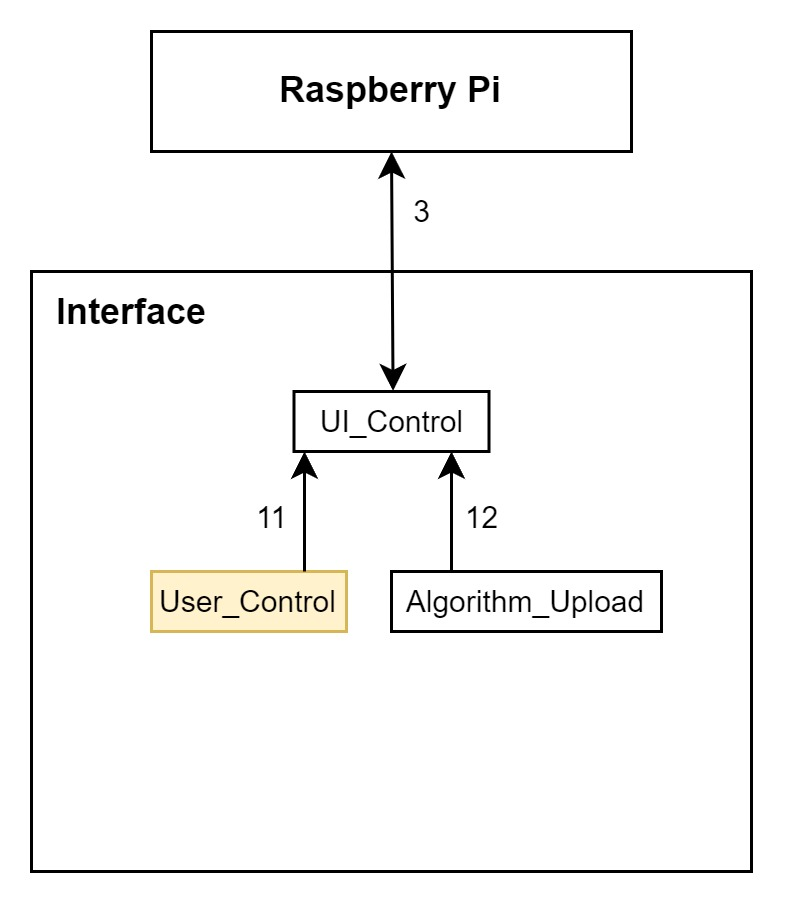
\includegraphics[width=0.60\textwidth]{images/interface/2_user.jpg}
 \caption{Interface Layer - User Control Subsystem}
\end{figure}

\subsubsection{Subsystem Programming Languages}
This subsystem is implemented using C, C++, and Python to efficiently process user commands and communicate with the motor control system.

\subsubsection{Subsystem Data Processing}
User inputs are converted into structured motion commands that control the rover's speed and direction. These commands are processed in real time to ensure responsiveness.

\newpage

\subsection{Algorithm Upload}
The Algorithm Upload subsystem allows users to upload pre-programmed pathfinding algorithms to enable autonomous navigation. It processes these algorithms and integrates them into the rover's control system, ensuring that the RoamBot can follow predefined paths without manual intervention.

\begin{figure}[h!]
	\centering
 	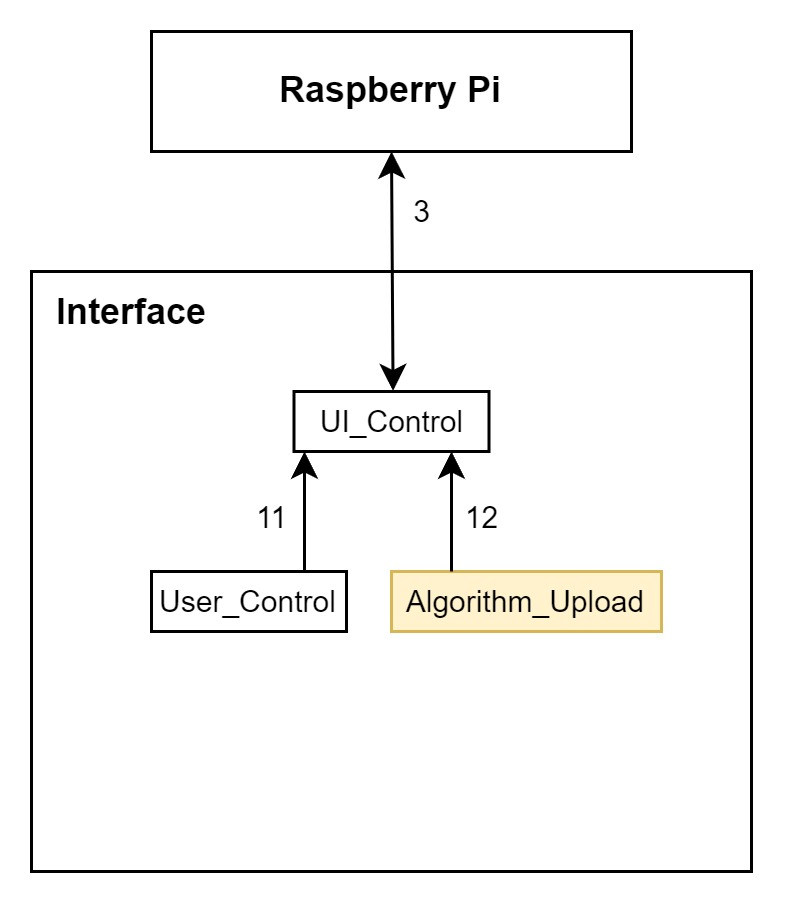
\includegraphics[width=0.60\textwidth]{images/interface/3_algorithm.jpg}
 \caption{Interface Layer - Algorithm Upload Subsystem}
\end{figure}

\subsubsection{Subsystem Data Structures}
The Algorithm Upload subsystem uses data structures like pathfinding grids or graphs to represent the environment, with nodes storing position and cost values values. The resulting path is stored as a sequence of waypoints.

\subsubsection{Subsystem Data Processing}
Data processing involves parsing the algorithm, running pathfinding algorithms like A* to generate a path, and converting it into motion commands. These commands are then sent as ROS2 messages to the motor control system for autonomous navigation.
